
\begin{figure}[ht]
    \centering
    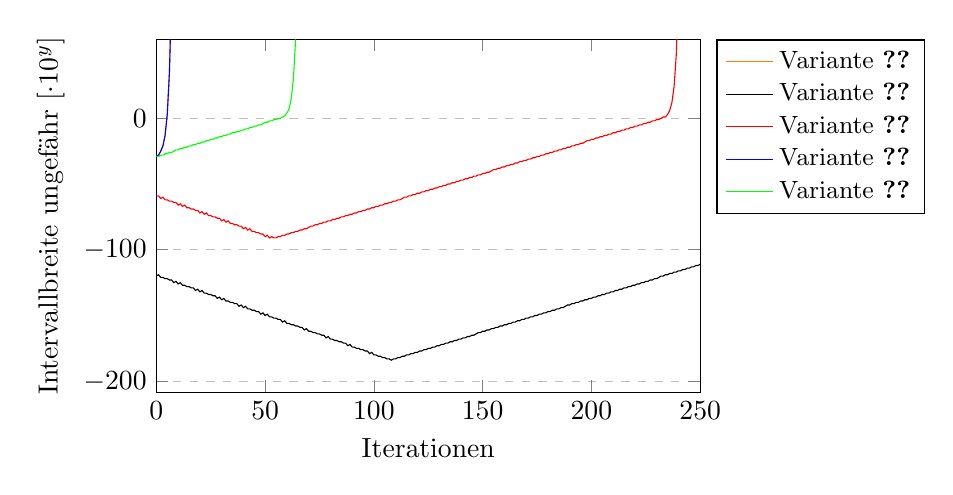
\begin{tikzpicture}
    \begin{axis}[
        width=0.7\textwidth,
        height=0.5\textwidth,
        xlabel={Iterationen},
        ylabel={Intervallbreite ungefähr $[\cdot 10^y ]$},
        legend pos=north west,
        xmin=0,xmax=250,
        ymax=60,
        ymajorgrids=true,
        grid style=dashed,
        legend pos=outer north east
    ]
    
    \addplot[
        color=orange,
        ]
        coordinates {
    (0,-29)
(1,-28)
(2,-25)
(3,-21)
(4,-13)
(5,03)
(6,35)
(7,97)
(8,223)
        };
        \addlegendentry{\small{Variante \ref{tm1}}}
    
    \addplot[
        color=black,
        ]
        coordinates {
    (0,-120) (1,-119) (2,-121) (3,-121) (4,-122) (5,-122) (6,-123) (7,-123) (8,-125) (9,-124) (10,-126) (11,-125) (12,-127) (13,-127) (14,-128) (15,-128) (16,-129) (17,-129) (18,-131) (19,-130) (20,-132) (21,-131) (22,-133) (23,-133) (24,-134) (25,-134) (26,-135) (27,-135) (28,-137) (29,-136) (30,-138) (31,-137) (32,-139) (33,-139) (34,-140) (35,-140) (36,-141) (37,-141) (38,-143) (39,-142) (40,-144) (41,-143) (42,-145) (43,-145) (44,-146) (45,-146) (46,-147) (47,-147) (48,-149) (49,-148) (50,-150) (51,-149) (52,-151) (53,-151) (54,-152) (55,-152) (56,-153) (57,-153) (58,-155) (59,-154) (60,-156) (61,-156) (62,-157) (63,-157) (64,-158) (65,-158) (66,-159) (67,-159) (68,-161) (69,-160) (70,-162) (71,-162) (72,-163) (73,-163) (74,-164) (75,-164) (76,-165) (77,-165) (78,-167) (79,-166) (80,-168) (81,-168) (82,-169) (83,-169) (84,-170) (85,-170) (86,-171) (87,-171) (88,-173) (89,-172) (90,-174) (91,-174) (92,-175) (93,-175) (94,-176) (95,-176) (96,-177) (97,-177) (98,-179) (99,-178) (100,-180) (101,-180) (102,-181) (103,-181) (104,-182) (105,-182) (106,-183) (107,-183) (108,-184) (109,-183) (110,-183) (111,-182) (112,-182) (113,-181) (114,-181) (115,-180) (116,-180) (117,-179) (118,-179) (119,-178) (120,-178) (121,-177) (122,-177) (123,-176) (124,-176) (125,-175) (126,-175) (127,-174) (128,-174) (129,-173) (130,-173) (131,-172) (132,-172) (133,-171) (134,-171) (135,-170) (136,-170) (137,-169) (138,-169) (139,-168) (140,-168) (141,-167) (142,-167) (143,-166) (144,-166) (145,-165) (146,-165) (147,-164) (148,-163) (149,-163) (150,-162) (151,-162) (152,-161) (153,-161) (154,-160) (155,-160) (156,-159) (157,-159) (158,-158) (159,-158) (160,-157) (161,-157) (162,-156) (163,-156) (164,-155) (165,-155) (166,-154) (167,-154) (168,-153) (169,-153) (170,-152) (171,-152) (172,-151) (173,-151) (174,-150) (175,-150) (176,-149) (177,-149) (178,-148) (179,-148) (180,-147) (181,-147) (182,-146) (183,-146) (184,-145) (185,-145) (186,-144) (187,-144) (188,-143) (189,-142) (190,-142) (191,-141) (192,-141) (193,-140) (194,-140) (195,-139) (196,-139) (197,-138) (198,-138) (199,-137) (200,-137) (201,-136) (202,-136) (203,-135) (204,-135) (205,-134) (206,-134) (207,-133) (208,-133) (209,-132) (210,-132) (211,-131) (212,-131) (213,-130) (214,-130) (215,-129) (216,-129) (217,-128) (218,-128) (219,-127) (220,-127) (221,-126) (222,-126) (223,-125) (224,-125) (225,-124) (226,-124) (227,-123) (228,-123) (229,-122) (230,-122) (231,-121) (232,-120) (233,-120) (234,-119) (235,-119) (236,-118) (237,-118) (238,-117) (239,-117) (240,-116) (241,-116) (242,-115) (243,-115) (244,-114) (245,-114) (246,-113) (247,-113) (248,-112) (249,-112) (250,-111)
        };
        \addlegendentry{\small{Variante \ref{tm2}}}
        
    \addplot[
        color=red,
        ]
        coordinates {
    (0,-59) (1,-59) (2,-61) (3,-60) (4,-62) (5,-62) (6,-63) (7,-63) (8,-64) (9,-64) (10,-66) (11,-65) (12,-67) (13,-66) (14,-68) (15,-68) (16,-69) (17,-69) (18,-70) (19,-70) (20,-72) (21,-71) (22,-73) (23,-72) (24,-74) (25,-74) (26,-75) (27,-75) (28,-76) (29,-76) (30,-78) (31,-77) (32,-79) (33,-78) (34,-80) (35,-80) (36,-81) (37,-81) (38,-82) (39,-82) (40,-84) (41,-83) (42,-85) (43,-84) (44,-86) (45,-86) (46,-87) (47,-87) (48,-88) (49,-88) (50,-90) (51,-89) (52,-91) (53,-90) (54,-91) (55,-91) (56,-90) (57,-90) (58,-89) (59,-89) (60,-88) (61,-88) (62,-87) (63,-87) (64,-86) (65,-86) (66,-85) (67,-85) (68,-84) (69,-84) (70,-83) (71,-82) (72,-82) (73,-81) (74,-81) (75,-80) (76,-80) (77,-79) (78,-79) (79,-78) (80,-78) (81,-77) (82,-77) (83,-76) (84,-76) (85,-75) (86,-75) (87,-74) (88,-74) (89,-73) (90,-73) (91,-72) (92,-72) (93,-71) (94,-71) (95,-70) (96,-70) (97,-69) (98,-69) (99,-68) (100,-68) (101,-67) (102,-67) (103,-66) (104,-66) (105,-65) (106,-65) (107,-64) (108,-64) (109,-63) (110,-63) (111,-62) (112,-62) (113,-61) (114,-60) (115,-60) (116,-59) (117,-59) (118,-58) (119,-58) (120,-57) (121,-57) (122,-56) (123,-56) (124,-55) (125,-55) (126,-54) (127,-54) (128,-53) (129,-53) (130,-52) (131,-52) (132,-51) (133,-51) (134,-50) (135,-50) (136,-49) (137,-49) (138,-48) (139,-48) (140,-47) (141,-47) (142,-46) (143,-46) (144,-45) (145,-45) (146,-44) (147,-44) (148,-43) (149,-43) (150,-42) (151,-42) (152,-41) (153,-41) (154,-40) (155,-39) (156,-39) (157,-38) (158,-38) (159,-37) (160,-37) (161,-36) (162,-36) (163,-35) (164,-35) (165,-34) (166,-34) (167,-33) (168,-33) (169,-32) (170,-32) (171,-31) (172,-31) (173,-30) (174,-30) (175,-29) (176,-29) (177,-28) (178,-28) (179,-27) (180,-27) (181,-26) (182,-26) (183,-25) (184,-25) (185,-24) (186,-24) (187,-23) (188,-23) (189,-22) (190,-22) (191,-21) (192,-21) (193,-20) (194,-20) (195,-19) (196,-19) (197,-18) (198,-17) (199,-17) (200,-16) (201,-16) (202,-15) (203,-15) (204,-14) (205,-14) (206,-13) (207,-13) (208,-12) (209,-12) (210,-11) (211,-11) (212,-10) (213,-10) (214,-9) (215,-9) (216,-8) (217,-8) (218,-7) (219,-7) (220,-6) (221,-6) (222,-5) (223,-5) (224,-4) (225,-4) (226,-3) (227,-3) (228,-2) (229,-2) (230,-1) (231,-1) (232,00) (233,01) (234,01) (235,03) (236,06) (237,12) (238,24) (239,48) (240,96)
        };
        \addlegendentry{\small{Variante \ref{tm3}}}
    
    
    \addplot[
        color=blue,
        ]
        coordinates {
    (0,-29) (1,-28) (2,-25) (3,-21) (4,-13) (5,03) (6,35) (7,97)
        };
        \addlegendentry{\small{Variante \ref{tm4}}}
    
    \addplot[
        color=green,
        ]
        coordinates {
    (0,-29) (1,-29) (2,-28) (3,-28) (4,-27) (5,-27) (6,-26) (7,-26) (8,-25) (9,-24) (10,-24) (11,-23) (12,-23) (13,-22) (14,-22) (15,-21) (16,-21) (17,-20) (18,-20) (19,-19) (20,-19) (21,-18) (22,-18) (23,-17) (24,-17) (25,-16) (26,-16) (27,-15) (28,-15) (29,-14) (30,-14) (31,-13) (32,-13) (33,-12) (34,-12) (35,-11) (36,-11) (37,-10) (38,-10) (39,-9) (40,-9) (41,-8) (42,-8) (43,-7) (44,-7) (45,-6) (46,-6) (47,-5) (48,-5) (49,-4) (50,-3) (51,-3) (52,-2) (53,-2) (54,-1) (55,-1) (56,00) (57,00) (58,01) (59,02) (60,04) (61,07) (62,15) (63,30) (64,60)
        };
        \addlegendentry{\small{Variante \ref{tm5}}}
                                      
    
    
    
    
    \end{axis}
    \end{tikzpicture}
    \caption{Größenordnung der Breite des Kernintervalls bei der Berechnung von $x_{250}$ mit Sweeping square\_only mit unterschiedlichen Definitionen des Taylormodells für $x_0$}
    \label{fig:strategy2}
\end{figure}